%%%%%%%%%%%%%%%%%%%%%%%%%%%%%%%%%%%%%%%%%
% University Assignment Title Page 
% LaTeX Template
% Version 1.0 (27/12/12)
%
% This template has been downloaded from:
% http://www.LaTeXTemplates.com
%
% Original author:
% WikiBooks (http://en.wikibooks.org/wiki/LaTeX/Title_Creation)
%
% License:
% CC BY-NC-SA 3.0 (http://creativecommons.org/licenses/by-nc-sa/3.0/)
% 
% Instructions for using this template:
% This title page is capable of being compiled as is. This is not useful for 
% including it in another document. To do this, you have two options: 
%
% 1) Copy/paste everything between \begin{document} and \end{document} 
% starting at \begin{titlepage} and paste this into another LaTeX file where you 
% want your title page.
% OR
% 2) Remove everything outside the \begin{titlepage} and \end{titlepage} and 
% move this file to the same directory as the LaTeX file you wish to add it to. 
% Then add \input{./title_page_1.tex} to your LaTeX file where you want your
% title page.
%
%%%%%%%%%%%%%%%%%%%%%%%%%%%%%%%%%%%%%%%%%
%\title{Title page with logo}
%----------------------------------------------------------------------------------------
%	PACKAGES AND OTHER DOCUMENT CONFIGURATIONS
%----------------------------------------------------------------------------------------

\documentclass[12pt]{article}
\usepackage[english]{babel}
\usepackage[utf8x]{inputenc}
\usepackage{amsmath}
\usepackage{graphicx}
\usepackage{url}
\usepackage[colorinlistoftodos]{todonotes}

\begin{document}

\begin{titlepage}

\newcommand{\HRule}{\rule{\linewidth}{0.5mm}} % Defines a new command for the horizontal lines, change thickness here

\center % Center everything on the page
 
%----------------------------------------------------------------------------------------
%	HEADING SECTIONS
%----------------------------------------------------------------------------------------

\textsc{\LARGE Politenico di Milano}\\[1.5cm] % Name of your university/college
\textsc{\Large Dipartimento Elettronica, Informazione e Bioingegneria}\\[0.5cm] % Major heading such as course name
\textsc{\large HEAPLab Project Report}\\[0.5cm] % Minor heading such as course title

%----------------------------------------------------------------------------------------
%	TITLE SECTION
%----------------------------------------------------------------------------------------

\HRule \\[0.4cm]
{ \huge \bfseries OpenCV people detection algorithm for Barbeque RTRM}\\[0.4cm] % Title of your document
\HRule \\[1.5cm]
 
%----------------------------------------------------------------------------------------
%	AUTHOR SECTION
%----------------------------------------------------------------------------------------

\begin{minipage}{0.4\textwidth}
\begin{flushleft} \large
\emph{Author:}\\
Giovanni \textsc{Lupi} % Your name
\end{flushleft}
\end{minipage}
~
\begin{minipage}{0.4\textwidth}
\begin{flushright} \large
\emph{Supervisor:} \\
Dr. Giusppe \textsc{Massari} % Supervisor's Name
\end{flushright}
\end{minipage}\\[2cm]

% If you don't want a supervisor, uncomment the two lines below and remove the section above
%\Large \emph{Author:}\\
%John \textsc{Smith}\\[3cm] % Your name

%----------------------------------------------------------------------------------------
%	DATE SECTION
%----------------------------------------------------------------------------------------

{\large \today}\\[2cm] % Date, change the \today to a set date if you want to be precise

%----------------------------------------------------------------------------------------
%	LOGO SECTION
%----------------------------------------------------------------------------------------


\includegraphics[width=100pt]{heaplogo.pdf}\\[1cm] % Include a department/university logo - this will require the graphicx package
 
%----------------------------------------------------------------------------------------

\vfill % Fill the rest of the page with whitespace

\end{titlepage}




\begin{abstract}
The aim of this project is to port the sample "peopledetect" from the
OpenCV library to the Barbeque Run-Time Resource Manager
(BarbequeRTRM).
OpenCV is a multiplaform library for real-time Computer Vision.
Given a source video file, the peopledetect application provides
an implementation for detecting people present in the scene.
Porting this sample to BarbequeRTRM allows the application to run
accordingly to the run-time managed Adaptive Execution Model.
This allows in turn the application to adjust its performances
according to the assigned computing resources.
\end{abstract}

\section{Introduction}

\subsection{Goals}

The goal of the present project is to port a sample application of
the OpenCV library to the Barbeque Run-Time Resource Manager. In
accordance with the project specifications, the "peopledetect"
sample was chosen.

Peopledetect is an application that shows an implementation of
an efficient method to detect humans in an image or a video.
This implementation is called Histogram of Oriented Gradients (HOG)
and will be described in the next few sections of the paper.
Porting this sample to BarbequeRTRM allows the
application to run accordingly to the run-time managed Adaptive
Execution Model. This allows in turn the application to adjust its
performances according to the assigned computing resources.

\subsection{OpenCV}
OpenCV (Open Source Computer Vision Library) is an open source library
that includes hundreds of computer vision algorithms. It mainly focuses
on image processing, video capture and analysis including features like face
detection and object detection.

The library is also cross-platform, supporting different programming
languages such as C++, Python and Java.
The present project was developed in C++ using version 3.2
of the library.

\subsection{People detection}
Object detection is a computer vision technique that allows to
identify and locate objects in an image or video. Specifically,
object detection creates bounding boxes around the detected objects,
allowing us to locate where they are or how they move
through a given scene.  Peopledetect is a sample of the OpenCV
library that is specifically tailored to detect pedestrians.
Therefore, the application will receive as input a video file
featuring one or more pedestrians, and will generate one or more
bounding boxes surronding the detected people.
There are several approaches that can be used to perform object
detection. Poepledetect employs a machine learning algorithm named
Histogram of Oriented Gradients (HOG).

\subsection{Histogram of Oriented Gradients}
The Histogram of Oriented Gradients is a feature descriptor. This is
an algorithm that produces a description of the visual features of
the input image or video by extracting useful information and
discarding the unnecessary information.  A HOG descriptor converts
an image into a feature vector of a certain length. In particular,
the features employed are the distribution of directions of
gradients.

The feature vector produced is then used as input for an image
classification algorithm like Support Vector Machine (SVM).
More details about the implementation of this algorithm will be
provided in the implementation section.

Understanding the tunable parameters for the algorithm allows the
adjustment of the application performances according to the Adaptive
Execution Model.

\subsection{Adaptive Execution Model}
The Adaptive Execution Model drives the application through a
managed execution flow, characterized by:
\begin{itemize}
\item Resource-awareness: the application can configure itself
	according to the assigned computing resources.
\item Runtime performance monitoring and negotiation: the
	application can observe the current throughput and ask for
	more resources.
	The Peopledetect application will therefore be able to adjust its
	performances according to the resources assigned by
	the BarbequeRTRM.
\end{itemize}

\section{Installation and setup}
The development platform chosen for this project is 
Ubuntu 18.04 (bionic) LTS.

BarbequeRTRM was installed according to the instuctions at
https://bosp.deib.polimi.it/guide-user.html
using \$HOME/Work/BOSP as installation directory.

A couple of problems were found during installation,
mostly due to the fact that the name of some packages had changed:
\begin{itemize}
\item ncurses-dev $\rightarrow$ libncurses5-dev
\item premake $\rightarrow$ premake4
\item git-core $\rightarrow$ git
\end{itemize}

BarbequeRTRM was then configured as explained in the guide
and the system was rebooted.

As a starting point for the project, the sample
https://github.com/HEAPLab/aem-template
was used.
The project uses CMake as buildsystem and the Qt Creator IDE
was chosen as development environment since it has a good
support for CMake.

To summarize:
\begin{itemize}
\item Operating System: Ubuntu 18.04
\item IDE: QtCreator
\item Compiler: gcc (Ubuntu 7.5.0-3ubuntu1~18.04) 7.5.0
\item Library: OpenCV 3.2
\end{itemize}


\section{Design and Implementation}
The ported application provides the same functionalities as the
original sample, while complying with the Adaptive Execution Model.
In addition to the original functionalities, the new application is
also capable of adjusting its performances according to the
available resources. This new feature was implemented by exploiting
the tuning of some suitable parameters, which will be examined in
greater detail later in this paragraph.

\subsection{Original application}
Peopledetect can use as video source a
file or the computer's camera. This choice can be made by the user
through the command line. Once the source has been chosen, the
application runs the actual detection procedure.

The Detector class contains all the information required for the
detection. The detect function performs the
detection: it takes as input a frame from the source video and
outputs a vector of rectangles that circumscribe the individuals.
Detect is as a wrapper for another function, called
detectMultiScale which can run in two different modes:
\begin{itemize}
\item Daimler mode $\rightarrow$ More accurate detection but computationally expensive
\item Default mode $\rightarrow$ Less CPU intensive but less detection power
\end{itemize}

By default, the original Peopledetect application only uses the
default mode algorithm, and the Daimler mode can only be selected
manually.
The execution flow is contained in the main function and can be
summed up in this way:
\begin{verbatim}
initialize detection
while (there are frames)
{
    read a frame from the video
    detect people in the frame
    draw the frame with detections highlighted with bounding rectangles
}
\end{verbatim}

\subsection{Ported application}
The original application included all the control flow in the
main function; all the steps of the detection belonged to a "for" loop.

The main loop was therefore split in separate functions
(callbacks for BarbequeRTRM) in a separate class called
PeopleDetect (a subclass of bbque::rtlib::BbqueEXC):
\begin{itemize}
\item onSetup $\rightarrow$ set up video source and define Barbeque CPS goal
\item onConfigure $\rightarrow$ get and display Barbeque configuration parameters
\item onRun $\rightarrow$ process a single frame (detect and display)
\item onMonitor $\rightarrow$ check the performance and adjust the detector parameters accordingly
\item onSuspend $\rightarrow$ not used
\end{itemize}

The main() function now does the following:
\begin{verbatim}
    parse command line arguments
    set up Barbeque RTRM
    instantiate the PeopleDetect class in Barbeque
    start
\end{verbatim}

\subsection{Performance tuning}
After finishing the porting, some additional effort was put into
understanding how to tune the performance of the application.
The high level idea was to set a target performance and, whenever
below this threshold, allow the application to give up some of its
detection accuracy to improve its speed.

This tradeoff between speed and accuracy is especially important
when running the detector in real-time on resource constrained
devices. 
This goal was achieved by analyzing and tweaking the parameters of
the detectMultiScale function.

detectMultiScale has two key parameters that, if changed, can dramatically
impact both the speed and the accuracy of the application. These parameters
are:
\begin{itemize}
\item winStride $\rightarrow$ The winStride parameter is a 2-tuple
	that dictates the "step size" in both the x and y location
	of the sliding window. A sliding window is a
	rectangular region of fixed width and height that
	"slides" across an image.
	At each stop of the sliding window we (1) extract HOG features and
	(2) pass these features on to our Linear SVM for
	classification. The process of feature extraction
	and classifier decision is very computationally expensive.
	Clearly, the smaller the window size, the more windows will
	need to be evaluated, lowering dramatically the
	speed of the algorithm. On the other hand,
	increasing the value of winStride allows to reduce
	the computational burden.
\item scale $\rightarrow$ 
An image pyramid is a multi-scale representation of an image, as in
Figure~\ref{fig:pyramid}.
\begin{figure}
\centering
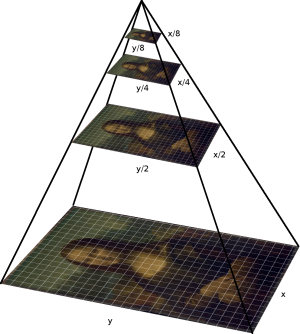
\includegraphics[width=0.5\textwidth]{pyramid_example.png}
\caption{\label{fig:pyramid}Pyramid example}
\end{figure}

At each layer of the image pyramid the image is downsized and (optionally)
smoothed via a Gaussian filter.

The scale parameter controls the factor in which the image is resized at each
layer of the image pyramid, ultimately influencing the number of levels in the
image pyramid.

A smaller scale will increase the number of layers in the image pyramid and
increase the amount of time it takes to process the image.
A larger scale will decrease the number of layers in the pyramid as
well as decrease the amount of time it takes to detect objects in an image.

\end{itemize}

Therefore, performance optimization was implemented as follows:
in the onSetup function a target CPS goal was set.
In onMonitor, the resulting CPS was examined and:
\begin{verbatim}
every 16 calls to onMonitor:
    if the CPS is substantially lower than the target CPS:
        switch from Daimler algorithm to default algorithm
        return
    if the CPS is lower than the target CPS:
        increase the scale by 0.02
        return
    OPTIONAL: increase the stride (not performed)
\end{verbatim}
The numeric values were determined experimentally.

\section{Experimental Results}

To test the performance of the ported code, the video file
\path{sample2.mp4} was used; the video shows people
walking in a station.
The video file was scaled from the original 1280x720 to a smaller
%%960x544 and
640x360,
because the original resolution was too challenging
for the available CPU resources.

A desired target CPS of 6 was determined empirically with some tests.
When the application starts, the Daimler HOG is used and the initial CPS is
\begin{verbatim}
PeopleDetect::onMonitor(): CPS=1.13868
\end{verbatim}
\begin{figure}
\centering
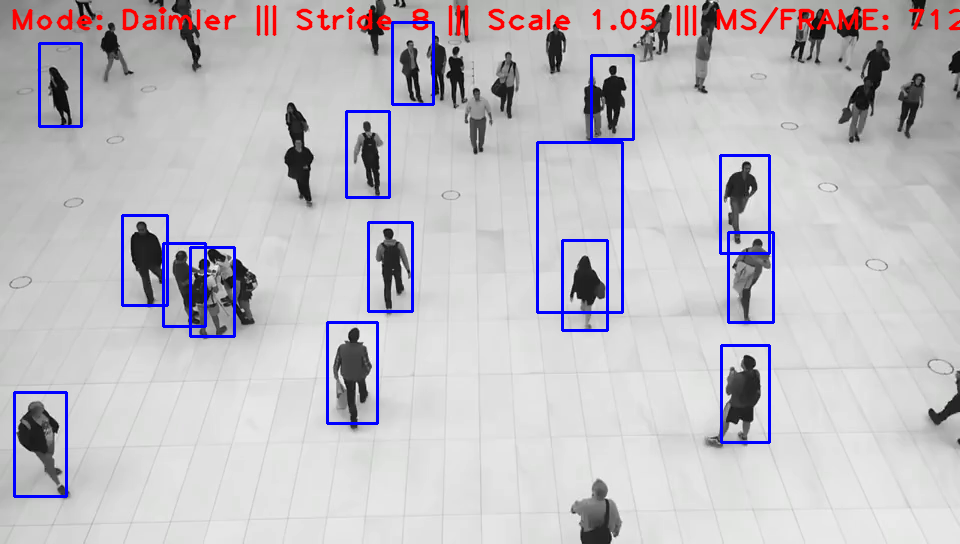
\includegraphics[width=1.0\textwidth]{peopledetect-0001.png}
\caption{\label{fig:peopledetect-0001}Daimler HOG with initial scale}
\end{figure}
After some cycles, the detection switches to the Default HOG and the performance
starts improving, at first without a noticeable loss of accuracy.
\begin{verbatim}
PeopleDetect::onMonitor(): CPS=2.21363
\end{verbatim}
At this point, the detection starts increasing the scale by 0.02 each time
until a maximum of 1.4 is reached. Beyond this point the Detector cannot detect
people any more.
A final
\begin{verbatim}
PeopleDetect::onMonitor(): CPS=4.65304
\end{verbatim}
\begin{figure}
\centering
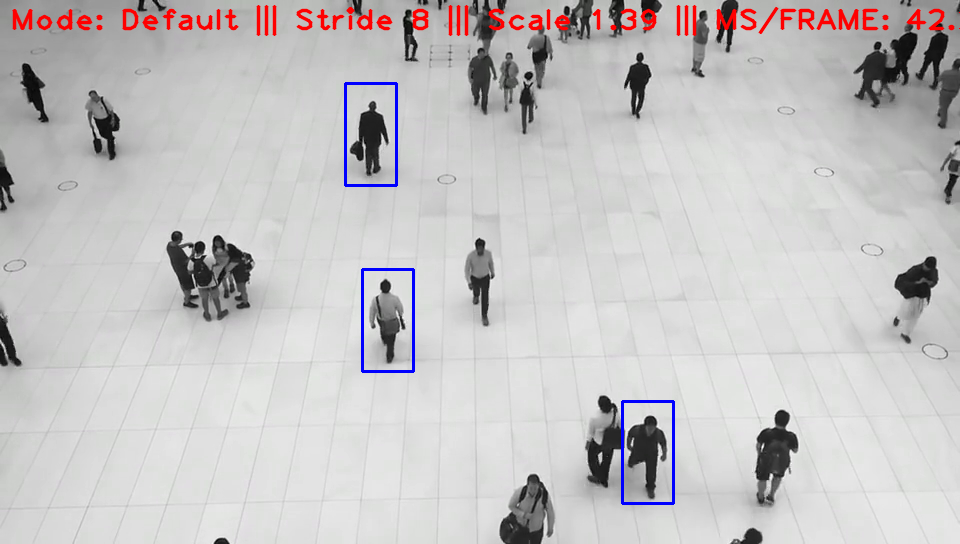
\includegraphics[width=1.0\textwidth]{peopledetect-0019.png}
\caption{\label{fig:peopledetect-0019}Default HOG with final scale}
\end{figure}
is reached, with a final performance which is 4 times the initial performance, at the
cost of dropping from 14 detected people to only 3 or 4.

The other tunable parameter, stride, was not modified by onMonitor, because
modifying both scale and stride at the same time led to a very fast loss of
detection.

\section{Conclusions}

The original "peopledetect" sample consisted of a main loop which analyzed a
video frame at a time in order to perform people detection.
This code organization
matched the application structure required by the BarbequeRTRM; the analysis of
the video frame was moved to the onRun() function of the environment, while the
preparatory steps became part of onSetup().

Optimizing the performance was more complex, mostly because the lack of documentation
of HOG detector,
and the effect of changes to the parameters had to be determined empirically.

In the end, a reasonable performance improvement through runtime adaptation of
the parameters was reached at the cost of a loss of precision in the detection.

\end{document}
